% Figure for MATH 591 §76 (Lecture 30), generated by courses/591/new/2026-11-13-L30/gen.py
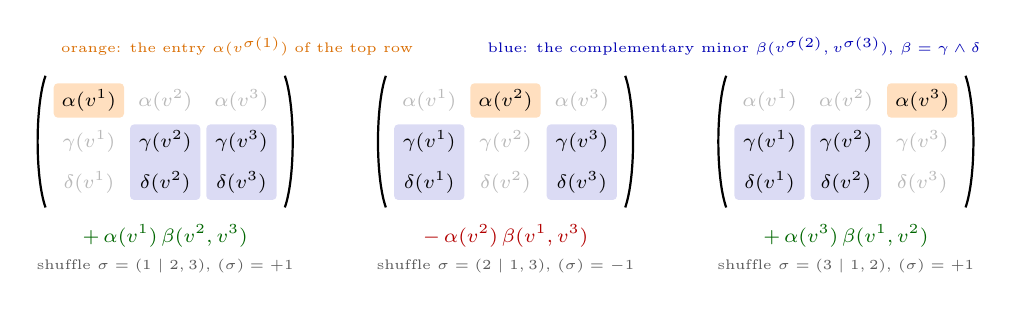
\begin{tikzpicture}[scale=0.95]
\fill[orange!25, rounded corners=1.5pt] (-0.470,-0.230) rectangle (0.470,0.230);
\fill[blue!70!black!14, rounded corners=1.5pt] (0.550,-1.330) rectangle (1.490,-0.320);
\fill[blue!70!black!14, rounded corners=1.5pt] (1.570,-1.330) rectangle (2.510,-0.320);
\node[font=\scriptsize, text=black] at (0.000,0.000) {$\alpha(v^{1})$};
\node[font=\scriptsize, text=gray!55] at (1.020,0.000) {$\alpha(v^{2})$};
\node[font=\scriptsize, text=gray!55] at (2.040,0.000) {$\alpha(v^{3})$};
\node[font=\scriptsize, text=gray!55] at (0.000,-0.550) {$\gamma(v^{1})$};
\node[font=\scriptsize, text=black] at (1.020,-0.550) {$\gamma(v^{2})$};
\node[font=\scriptsize, text=black] at (2.040,-0.550) {$\gamma(v^{3})$};
\node[font=\scriptsize, text=gray!55] at (0.000,-1.100) {$\delta(v^{1})$};
\node[font=\scriptsize, text=black] at (1.020,-1.100) {$\delta(v^{2})$};
\node[font=\scriptsize, text=black] at (2.040,-1.100) {$\delta(v^{3})$};
\draw[thick] (-0.580,0.330) .. controls (-0.720,-0.070) and (-0.720,-1.030) .. (-0.580,-1.430);
\draw[thick] (2.620,0.330) .. controls (2.760,-0.070) and (2.760,-1.030) .. (2.620,-1.430);
\node[font=\scriptsize, text=green!40!black] at (1.020,-1.810) {$+\,\alpha(v^{1})\,\beta(v^{2}, v^{3})$};
\node[font=\tiny, gray!70!black] at (1.020,-2.210) {shuffle $\sigma = (1 \mid 2, 3)$, $\sgn(\sigma) = + 1$};
\fill[orange!25, rounded corners=1.5pt] (5.100,-0.230) rectangle (6.040,0.230);
\fill[blue!70!black!14, rounded corners=1.5pt] (4.080,-1.330) rectangle (5.020,-0.320);
\fill[blue!70!black!14, rounded corners=1.5pt] (6.120,-1.330) rectangle (7.060,-0.320);
\node[font=\scriptsize, text=gray!55] at (4.550,0.000) {$\alpha(v^{1})$};
\node[font=\scriptsize, text=black] at (5.570,0.000) {$\alpha(v^{2})$};
\node[font=\scriptsize, text=gray!55] at (6.590,0.000) {$\alpha(v^{3})$};
\node[font=\scriptsize, text=black] at (4.550,-0.550) {$\gamma(v^{1})$};
\node[font=\scriptsize, text=gray!55] at (5.570,-0.550) {$\gamma(v^{2})$};
\node[font=\scriptsize, text=black] at (6.590,-0.550) {$\gamma(v^{3})$};
\node[font=\scriptsize, text=black] at (4.550,-1.100) {$\delta(v^{1})$};
\node[font=\scriptsize, text=gray!55] at (5.570,-1.100) {$\delta(v^{2})$};
\node[font=\scriptsize, text=black] at (6.590,-1.100) {$\delta(v^{3})$};
\draw[thick] (3.970,0.330) .. controls (3.830,-0.070) and (3.830,-1.030) .. (3.970,-1.430);
\draw[thick] (7.170,0.330) .. controls (7.310,-0.070) and (7.310,-1.030) .. (7.170,-1.430);
\node[font=\scriptsize, text=red!70!black] at (5.570,-1.810) {$-\,\alpha(v^{2})\,\beta(v^{1}, v^{3})$};
\node[font=\tiny, gray!70!black] at (5.570,-2.210) {shuffle $\sigma = (2 \mid 1, 3)$, $\sgn(\sigma) = - 1$};
\fill[orange!25, rounded corners=1.5pt] (10.670,-0.230) rectangle (11.610,0.230);
\fill[blue!70!black!14, rounded corners=1.5pt] (8.630,-1.330) rectangle (9.570,-0.320);
\fill[blue!70!black!14, rounded corners=1.5pt] (9.650,-1.330) rectangle (10.590,-0.320);
\node[font=\scriptsize, text=gray!55] at (9.100,0.000) {$\alpha(v^{1})$};
\node[font=\scriptsize, text=gray!55] at (10.120,0.000) {$\alpha(v^{2})$};
\node[font=\scriptsize, text=black] at (11.140,0.000) {$\alpha(v^{3})$};
\node[font=\scriptsize, text=black] at (9.100,-0.550) {$\gamma(v^{1})$};
\node[font=\scriptsize, text=black] at (10.120,-0.550) {$\gamma(v^{2})$};
\node[font=\scriptsize, text=gray!55] at (11.140,-0.550) {$\gamma(v^{3})$};
\node[font=\scriptsize, text=black] at (9.100,-1.100) {$\delta(v^{1})$};
\node[font=\scriptsize, text=black] at (10.120,-1.100) {$\delta(v^{2})$};
\node[font=\scriptsize, text=gray!55] at (11.140,-1.100) {$\delta(v^{3})$};
\draw[thick] (8.520,0.330) .. controls (8.380,-0.070) and (8.380,-1.030) .. (8.520,-1.430);
\draw[thick] (11.720,0.330) .. controls (11.860,-0.070) and (11.860,-1.030) .. (11.720,-1.430);
\node[font=\scriptsize, text=green!40!black] at (10.120,-1.810) {$+\,\alpha(v^{3})\,\beta(v^{1}, v^{2})$};
\node[font=\tiny, gray!70!black] at (10.120,-2.210) {shuffle $\sigma = (3 \mid 1, 2)$, $\sgn(\sigma) = + 1$};
\node[font=\tiny, text=orange!85!black, anchor=west] at (-0.500,0.720) {orange: the entry $\alpha(v^{\sigma(1)})$ of the top row};
\node[font=\tiny, text=blue!70!black, anchor=west] at (5.200,0.720) {blue: the complementary minor $\beta(v^{\sigma(2)}, v^{\sigma(3)})$, $\beta = \gamma \wedge \delta$};
\end{tikzpicture}
